\section{Introduction}

% Introduce transformer / LLM / 
Transformers have revolutionized AI across various fields, including language, vision, and science~\cite{wei2022emergentabilitieslargelanguage,attention,kojima2023largelanguagemodelszeroshot}. Transformer-based autoregressive large language models (LLMs), like GPT~\cite{gpt4} and LLaMA~\cite{llama}, are now widely deployed in many applications, such as chatbots~\cite{chatgpt}, code generation~\cite{code_gen}, tool-use and computer-use workflows \cite{agentic_workflow}. 

The rapid rise of agentic capabilities of  LLMs, e.g.~computer-use~\cite{OmniParser}, tool-use~\cite{browser_use2024, WebVoyager}, and command-line agents~\cite{command_agent}, heavily relies on their ability to process and reason over very large context windows. For instance, command-line agents need to both comprehend and generate large-scale codebases~\cite{code_gen_long_context, multi-swe, LongCodeBench}, while tool- and computer-use agentic workflows must keep track of multiple pieces of information across prolonged inputs---such as a complete web page DOM---which typically require very long contexts \cite{webdom_long_context,workarena,BrowserGym}.
\Cref{fig:Workload_analysis} shows that, when compared to chatbot workloads, agentic workloads consume~100$\times$ more tokens per inference on average and up to~1,000$\times$ in extreme. In response, modern LLMs have delibrately expanded their context windows: the original GPT-3~\cite{gpt3} supports roughly 2K tokens, whereas GPT-4\cite{gpt4} reaches up to 32K tokens, and \llamaIVMVK\cite{llama4_maverick} to 1M tokens.

% In your document
\begin{figure}[t]
  \centering

  % ---------- Row 1: wide panel (cap height to fit the page) ----------
  \begin{subfigure}{\linewidth}
    \centering
    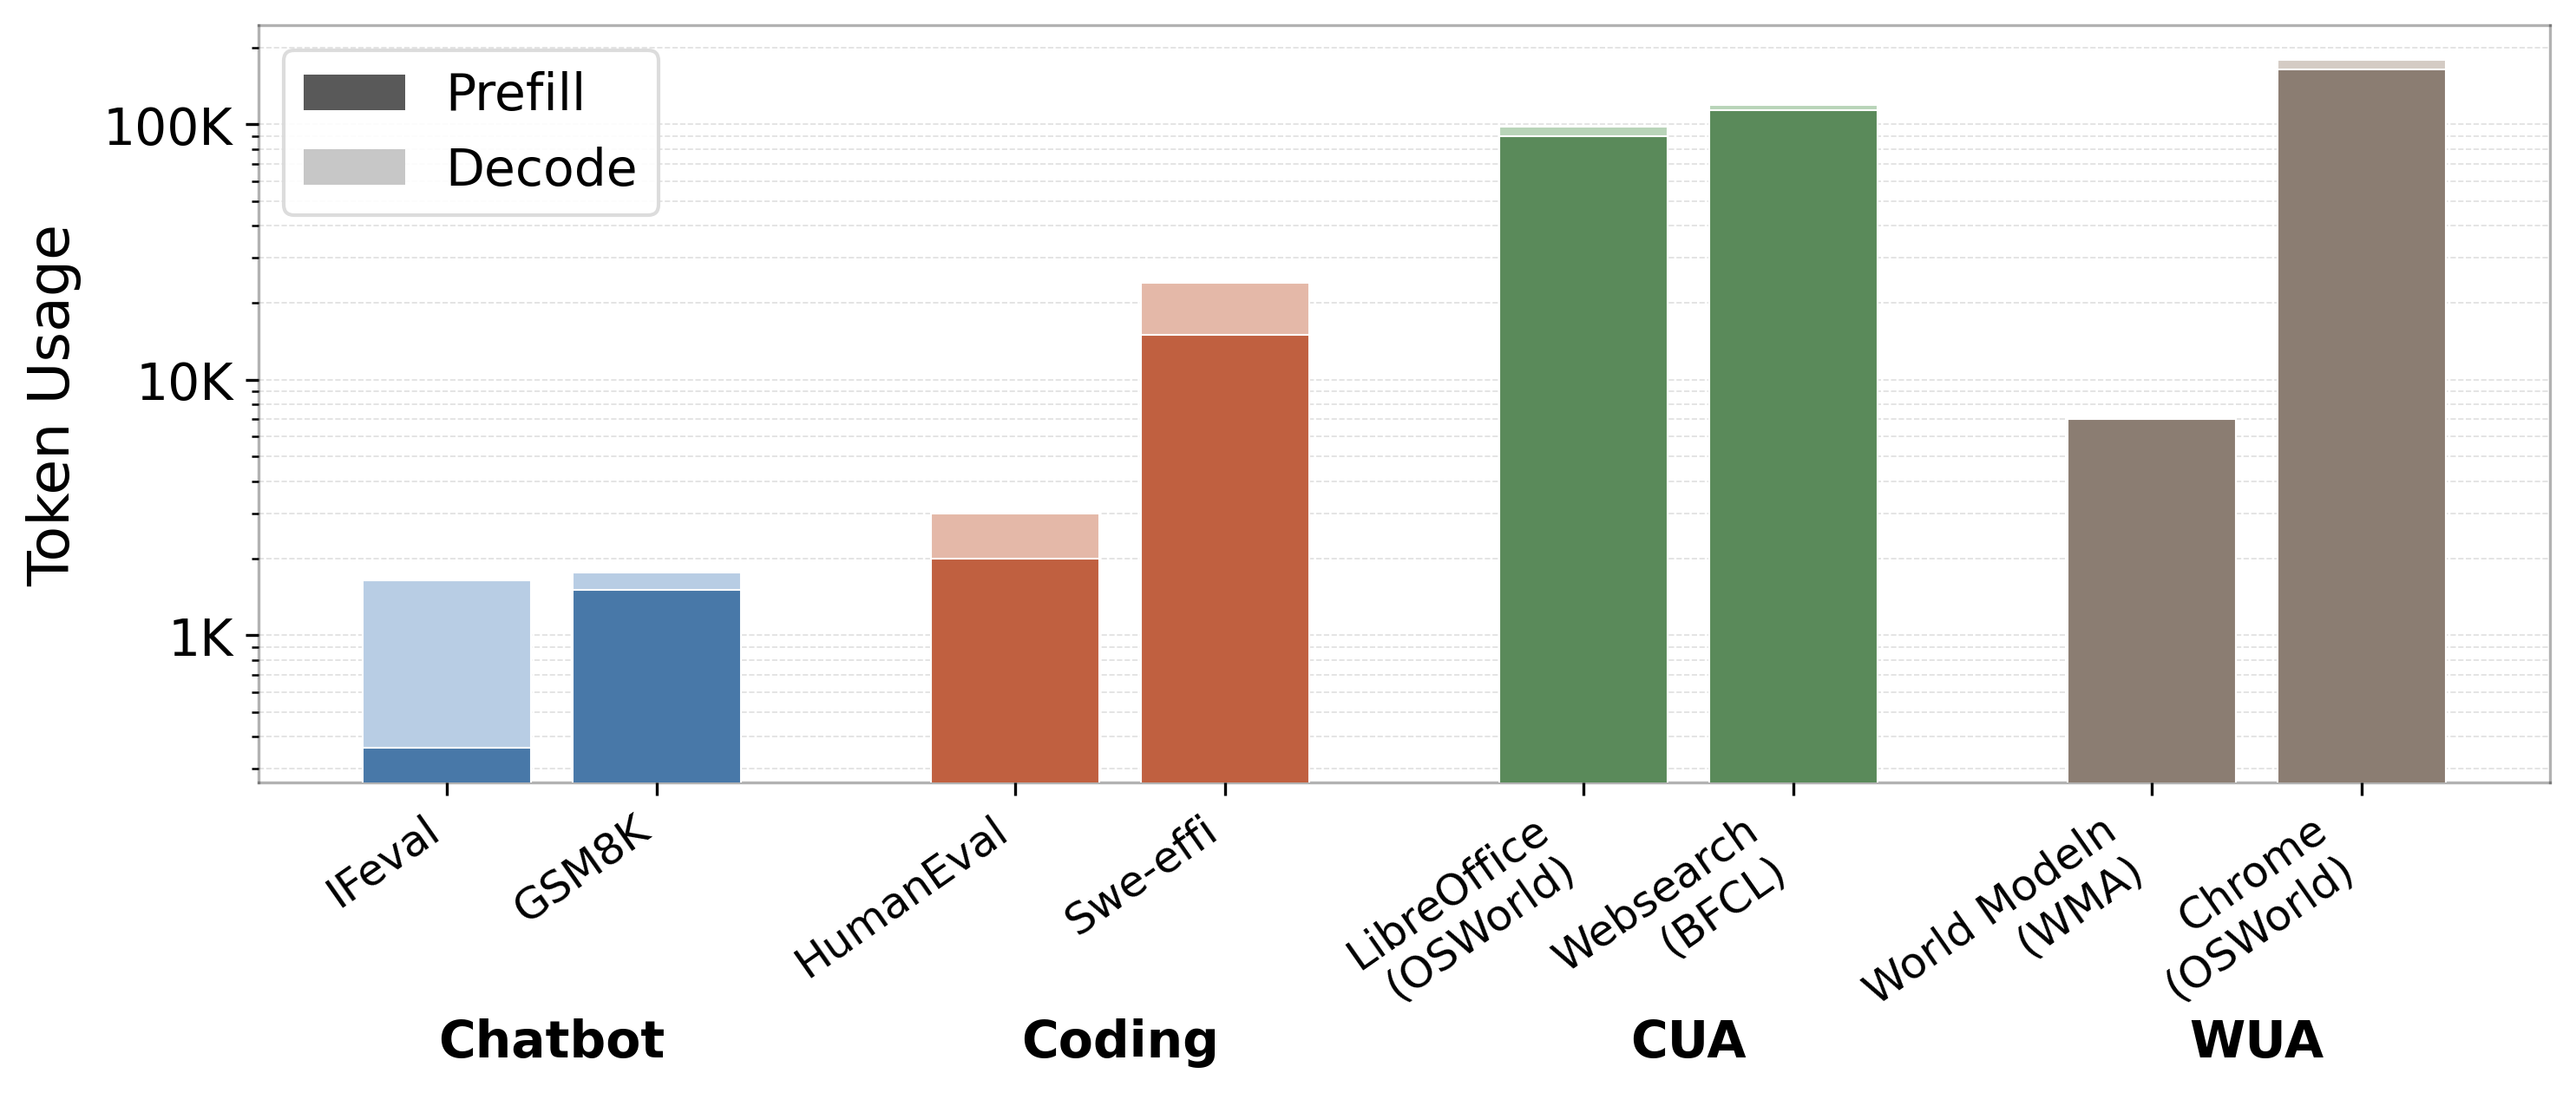
\includegraphics[width=\linewidth,height=0.30\textheight,keepaspectratio]{Figures/motivation_fig/workload_context_by_domain_bar_colors_chatbot.png}
    \caption{Token usage comparison across standard chatbot~\cite{ifeval,gsm8k}, coding~\cite{humaneval, sweeffi}, and agentic workloads, including Computer Use Agent (CUA)~\cite{osworld, agent_s2} and Web Use Agent (WUA)~\cite{webagent, osworld}.}
    \label{fig:Workload_analysis}
  \end{subfigure}

  \medskip

  % ---------- Row 2: two square-ish panels ----------
  \begin{subfigure}{0.48\linewidth}
    \centering
    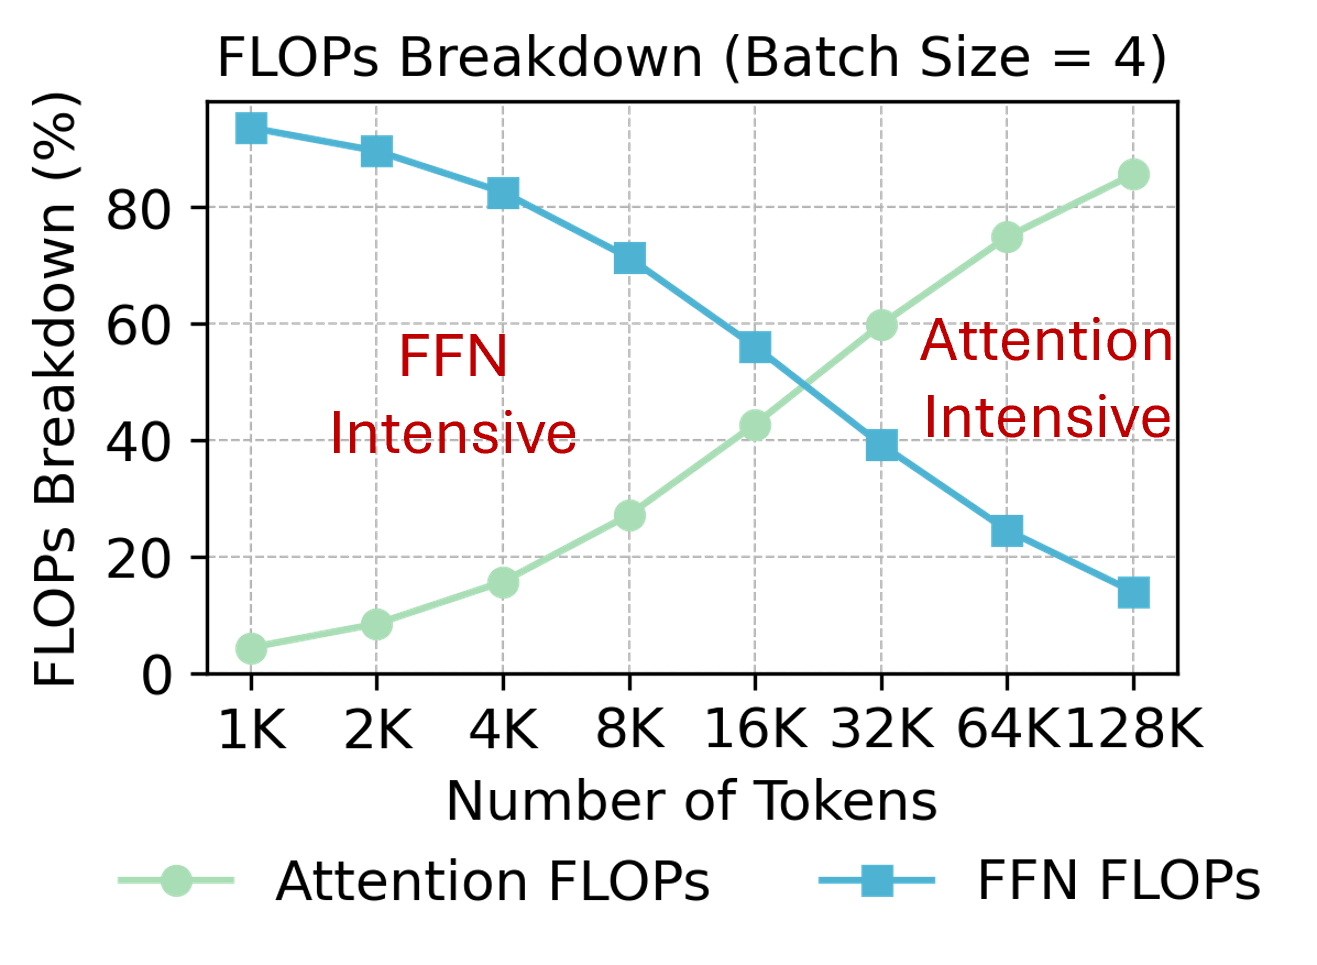
\includegraphics[width=\linewidth,height=0.22\textheight,keepaspectratio]{Figures/motivation_fig/Flops_breakdown.png}
    \caption{Compute intensity shifts from FFN to Attention blocks with an increasing context length.}
    \label{fig:Flops_breakdown}
  \end{subfigure}\hfill
  \begin{subfigure}{0.48\linewidth}
    \centering
    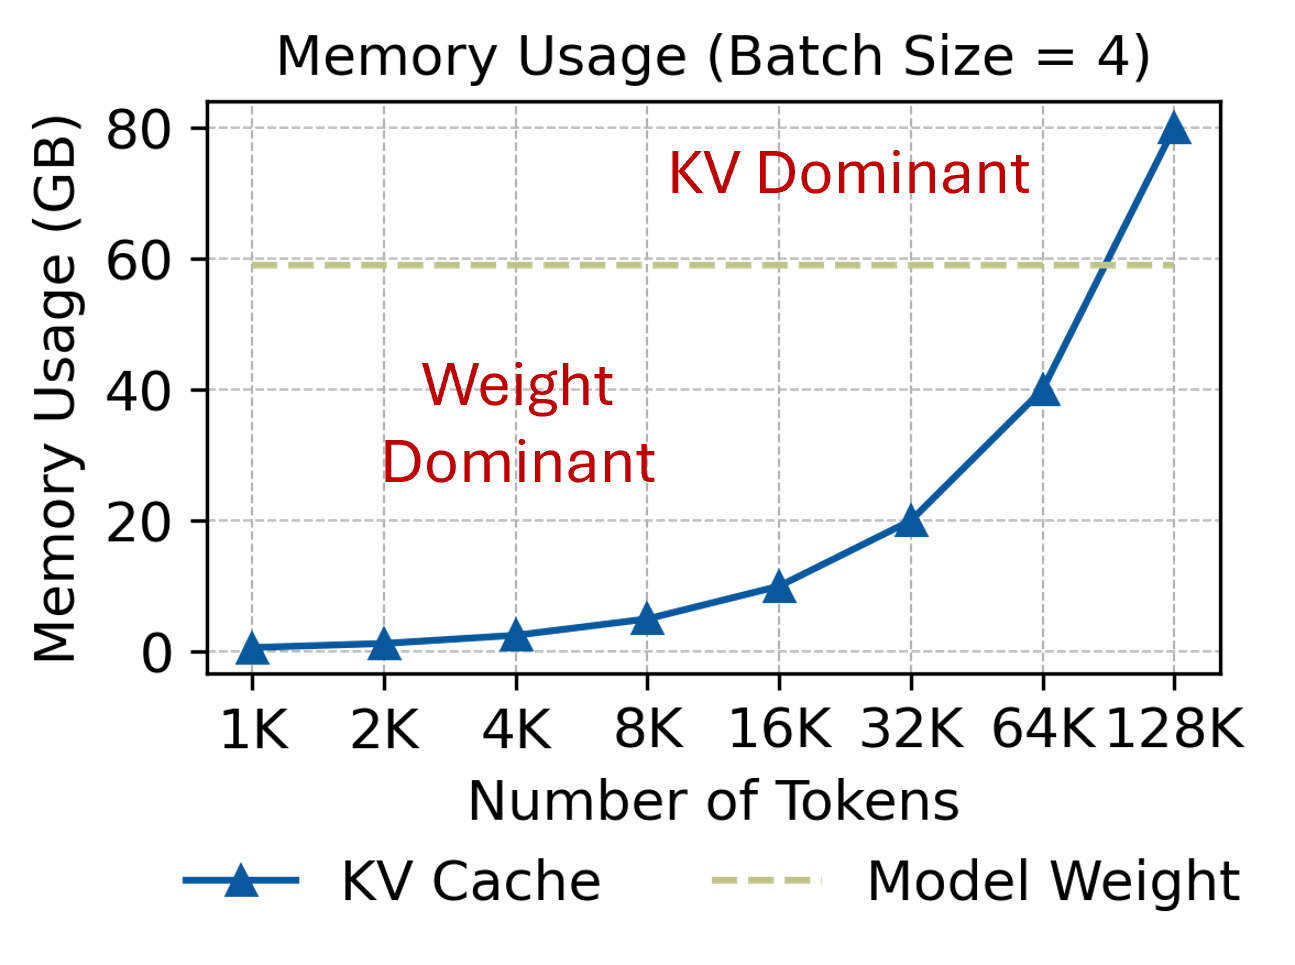
\includegraphics[width=\linewidth,height=0.22\textheight,keepaspectratio]{Figures/motivation_fig/Memory_usage.png}
    \caption{KV cache scales with context length, eventually dominates memory usage.}
    \label{fig:mem_utilization}
  \end{subfigure}
  \caption{An illustration of agentic inference workloads shows how they typically generate many more tokens per single inference run \subref{fig:Workload_analysis}, contain both FFN-compute-intensive and attention-compute-intensive phases \subref{fig:Flops_breakdown}, and include weight memory-capacity-dominant and KV-dominant phases \subref{fig:mem_utilization} within a single inference run.}
  \label{fig:two-layer-subfig}
  \vspace{-10pt}
\end{figure}


To clarify the computational impact of agentic workloads, \Cref{fig:Flops_breakdown} analyzes a \llamaIIIBig model with long-context capability and demonstrates that, when the number of generated tokens is small, the Feed-Forward Networks (FFNs) contribute most of the inference FLOPs. As the number of generated tokens increases, however, the attention layers gradually dominate FLOP counts. Because inference is autoregressive, these two computational phases naturally coexist within a single long-context decoding run. For example, in the LongWriter~\cite{longwriter} workload, the prefilling phase completes at around 5K tokens, after which the decoding phase expands the context to a large value -- 85K tokens. As the sequence grows, the computational intensity (in FLOPs) start to transition from FFN-dominated to attention-dominated, with the crossover occurring at roughly 19K generated tokens, as shown in \Cref{fig:Flops_breakdown}. This shift makes both FFN and attention layers practical and necessary targets for optimization.



Agentic LLM inference also consumes significant HBM resources.
\Cref{fig:mem_utilization} identifies two major limiting factors on the memory side. 
First, the large number of KV values and weights that must be read, together with the portion of KV values written back, impose substantial memory bandwidth demands. 
Second, as context length increases, the KV-cache requirement grows linearly, quickly increasing memory usage and often surpassing the size of the model weights, making HBM capacity a primary limiting factor.
For example, in \llamaIIIBig, at a 128k context~\cite{llama3}, the FP16 KV cache for a single batch is approximately 39 GB, which limits how many batches can be kept on the chip~\cite{AI_and_Mem_Wall}.
Building on this observation, we suggest that there are two main challenges on the off-chip memory side, namely, (i) the limited memory bandwidth and (ii) the restricted memory capacity.
We collectively term these \emph{memory walls}. Together, they prevent devices from reaching peak performance at inference time, consistent with observations in prior work~\cite{AI_and_Mem_Wall, Efficient_LLM_Inference, LLMCompass}.



The memory wall phenomenon leads to the underutilization of computing resources on modern hardware, such as TPUs and GPUs. This effect is particularly evident in compute units dedicated to General Matrix-Matrix Multiplication (GEMM) operations ($\mathbb{R}^{M \times K} \times \mathbb{R}^{K \times N} \to \mathbb{R}^{M \times N}$), denoted as $(M, K) \times (K, N)$, which constitute the core computational workload during LLM inference~\cite{Transistive}.
At the microarchitectural level, most hardware is built with square-shaped systolic arrays or matrix multiplication units, typically designed so that the $M$ and $N$ dimensions are close in size to $K$. For example, TPU v3~\cite{TPU_V3_Systolic_Array} features a 128×128 systolic array, supporting $M = K = N = 128$ GEMM operations. 
% The NVIDIA Blackwell B200 architecture~\cite{nvidia2024blackwell} introduces a minimal computation granularity of $64\times8\times16$.
However, in long-context agentic models, as shown in \Cref{fig:mem_utilization}, memory often becomes the primary constrain for the inference batch size. This results in a \textit{fat GEMM} operation, where the batch-related dimension (typically $M$ in $(M,K)\times(K,N)$) is much smaller than the other operating dimension. This essentially produces an uneven matrix shape\footnote{All KVs must be stored, so the batch size (the \(M\) dimension) is kept lower than the hidden size (\(K\)). While various offloading techniques are available~\cite{deepspeedinference}, they complicate system-level trade-offs and tend to make the system more memory I/O--bound.}. This imbalance hinders systolic arrays and Tensor Cores from achieving a high computational resources utilization rate~\cite{FlashDecoding}.



To this end, we propose the \textbf{P}rogrammable \textbf{L}ong-context \textbf{E}fficient \textbf{N}eural \textbf{A}ccelerator (PLENA), an efficient transformer model accelerator system designed to maintain high utilization of GEMM units across all inference stages (prefilling and decoding), particularly for agentic LLM inference tasks with large contexts. PLENA achieves high efficiency for long-context inference by exploring three optimization pathways across both hardware and software design spaces. 


\begin{figure}[t]
  \centering
  % Left subfigure
  \begin{subfigure}[t]{0.32\linewidth}
    \centering
    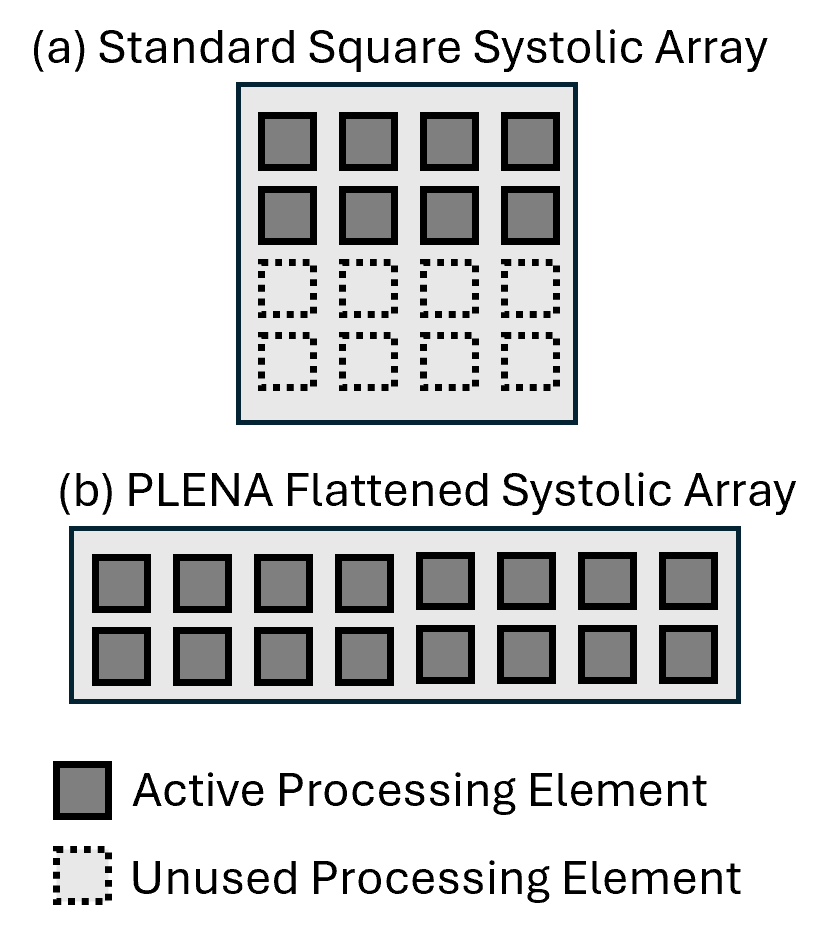
\includegraphics[width=\linewidth]{Figures/motivation_fig/Simp_SA_Comparison.png}
    \caption{PLENA achieves higher utilization than the standard square systolic array with the same resources.}
    \label{fig:sa_compare_plot}
  \end{subfigure}
  \hfill
  % Right subfigure
  \begin{subfigure}[t]{0.65\linewidth}
    \centering
    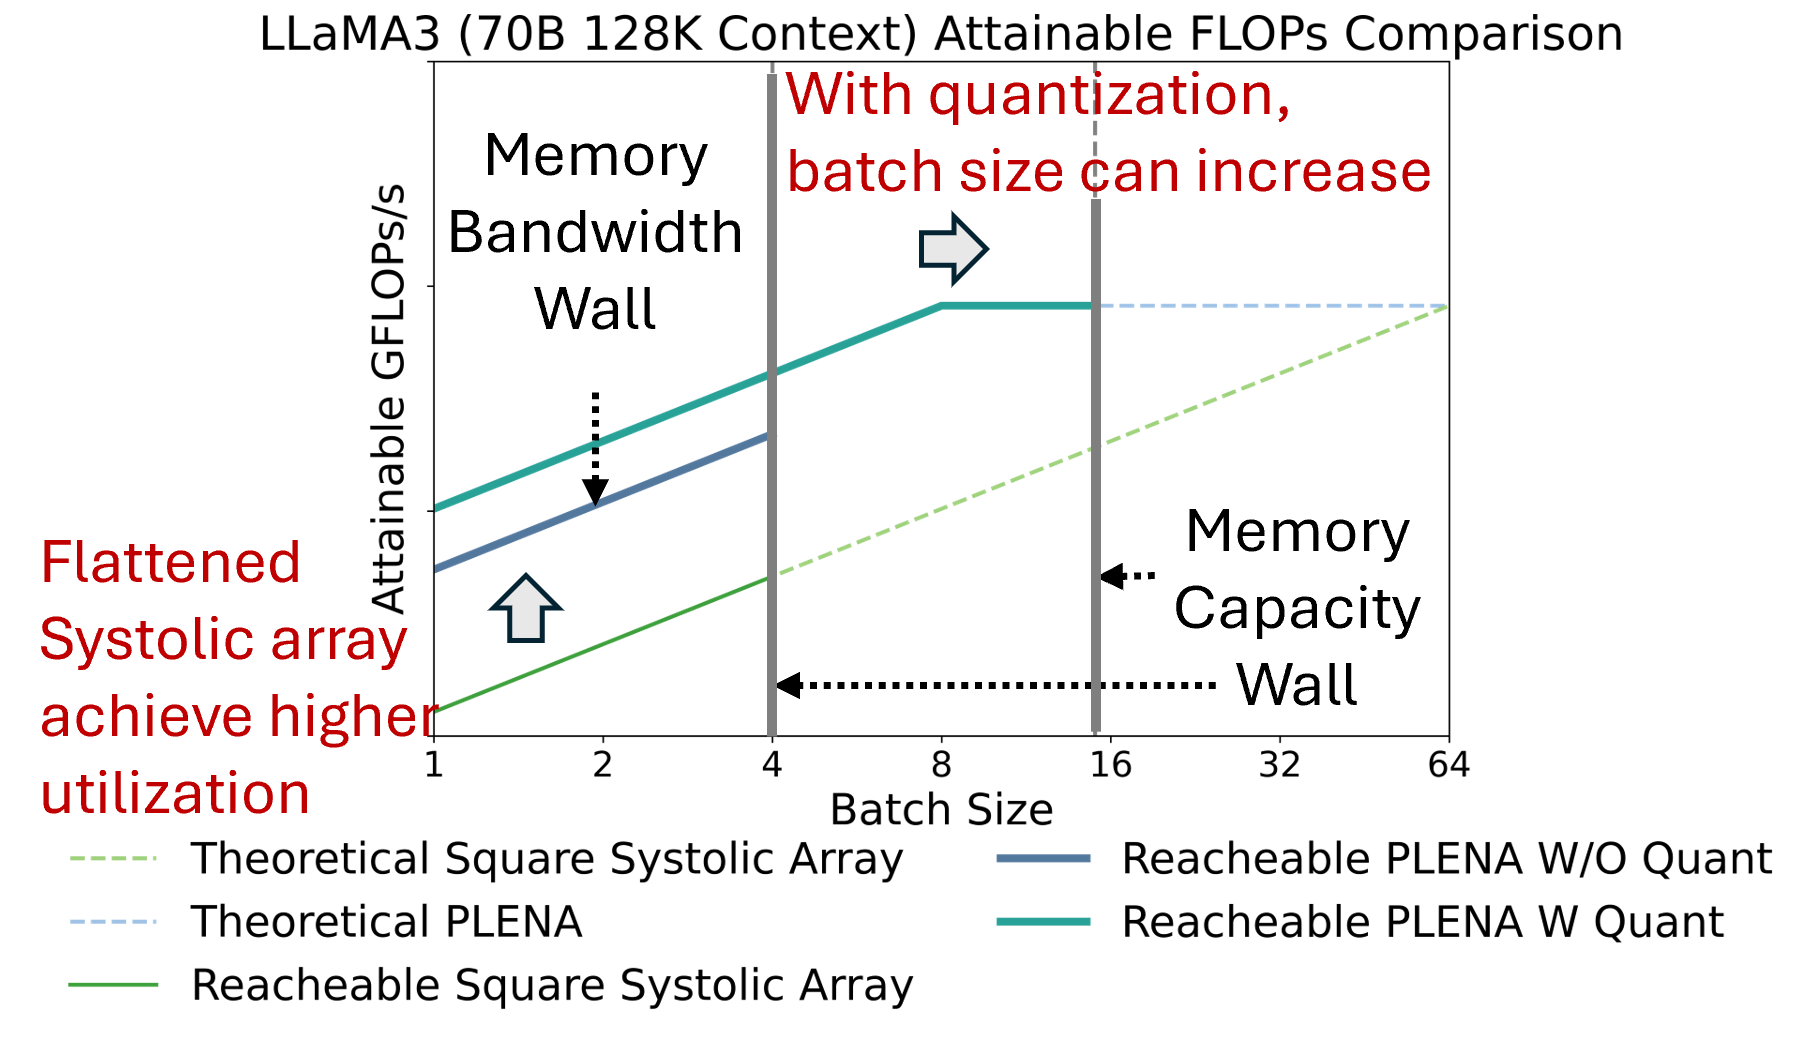
\includegraphics[width=\linewidth]{Figures/motivation_fig/GEMM_Utilization.png}
    \caption{PLENA’s optimization pathways---(1) a flattened systolic array and (2) asymmetric quantization---together achieve improved effective memory bandwidth utilization and help reduce memory capacity limitations.}
    \label{fig:sa_compare_analysis}
  \end{subfigure}

  \caption{A comparison of attainable FLOPs between a square-shaped systolic array (e.g.~TPUs) and PLENA’s when using the same number of multipliers\protect\footnotemark.}
  \label{fig:motivation}
  \vspace{-10pt}
\end{figure}


\footnotetext{64$\times$64 square-shaped systolic array and 8$\times$512 flattened systolic array. Data derived from 144\,GB HBM capacity and 512\,GB/s memory bandwidth.} First, our novel flattened systolic array (\textit{Pathway 1}) resolves the architectural mismatch caused by the typical square-shaped GEMM used for inference, achieving a higher compute utilization of multiplication resources as illustrated in \Cref{fig:sa_compare_plot,fig:sa_compare_analysis}. 
% The array can also be partitioned into multiple cores to maintain high utilization during per-head GEMM operations in the attention computation. 
Second, we apply an \textit{asymmetric quantization strategy} with Post-Training Quantization (PTQ) optimizations (\textit{Pathway~2}), where Weights(W)/Activations(A)/KV Cache(KV) can be set to different precisions to alleviate both memory bandwidth and capacity walls. 
With more aggressive W and KV cache quantization, we free up more space in HBM for data scaling (e.g., supporting larger batch sizes). 
% We also integrate , achieving superior performance compared to existing methods while effectively mitigating the two memory walls. 
\Cref{fig:motivation} shows how these pathways together can \textbf{increase the utilization} compared to the conventional square-shaped GEMM hardware without any optimization.
Finally, as \Cref{fig:Flops_breakdown} shows that attention dominates the compute at longer context lengths, we design PLENA’s custom ISA and novel architecture to effectively support FlashAttention (\textit{Pathway~3})—an IO-aware, fused attention algorithm that substantially reduces off-chip memory traffic~\cite{FlashAttention}. This reduces the likelihood of attention operations saturating memory bandwidth, thereby diminishing the wall’s effect.


Together, these optimization pathways yield significantly higher utilization than conventional square-shaped systolic-array accelerators. The main contributions are as follows:

\begin{itemize}[leftmargin=1em]
    \item We analytically characterize the bandwidth and capacity memory walls in agentic LLM inference and show that existing systolic-array accelerators are normally heavily under-utilized when running agentic workloads.

    \item We introduce three optimization pathways that jointly address the under-utilization caused by memory walls: (i)~a flattened systolic array architecture; (ii)~an asymmetric quantization scheme, coupled with an in-depth exploration of micro-scaling arithmetic's compatibility with optimization techniques such as rotation and norm-guided iterative optimization; and (iii)~a native support for FlashAttention. Together, these enable a holistic approach that addresses both bandwidth and capacity limitations by integrating hardware-level and algorithmic optimizations. 
    
    \item We present PLENA, a complete hardware–software system that realizes the above optimizations. PLENA integrates: (i)~a custom instruction set (PLENA\_ISA) for large Transformer inference; (ii)~a PyTorch-to-PLENA\_ISA compiler; (iii)~an HBM-enabled transactional simulator; (iv)~an automated, accuracy-aware design-space exploration (DSE) flow; and (v)~a full RTL implementation. We demonstrate that PLENA supports different SOTA transformer model variants (e.g., GQA, MHA and MLA~\cite{MLA}, Dense and MoE~\cite{MoE}). We also show that PLENA achieves superior efficiency for agentic LLM inference. Under identical multiplier counts and memory configurations during LLaMA agentic inference, PLENA delivers up to 2.23$\times$ and 4.70$\times$ higher throughput than the A100 GPU and TPU v6e, respectively, and up to 4.04$\times$ higher energy efficiency (Token/J) than the A100. The entire PLENA system will be fully open-sourced upon acceptance.
\end{itemize}

